\documentclass[sigconf]{acmart}

\AtBeginDocument{%
  \providecommand\BibTeX{{%
    \normalfont B\kern-0.5em{\scshape i\kern-0.25em b}\kern-0.8em\TeX}}}

\usepackage{dblfloatfix}
\usepackage{mathtools}
\usepackage{hyperref}
\usepackage[htt]{hyphenat}
\usepackage{listings}
\usepackage{xcolor}
\usepackage[framemethod=tikz]{mdframed}
\usepackage{algorithm}
\usepackage{algpseudocode}
\usepackage{float}
\usepackage{caption}
\usepackage{tikz}
\usetikzlibrary{shapes,arrows,arrows.meta}

\definecolor{codegreen}{rgb}{0,0.6,0}
\definecolor{codegray}{rgb}{0.5,0.5,0.5}
\definecolor{codepurple}{rgb}{0.58,0,0.82}
\definecolor{backcolour}{rgb}{0.95,0.95,0.92}

\lstdefinestyle{mystyle}{
	backgroundcolor=\color{backcolour},
	commentstyle=\color{codegreen},
	keywordstyle=\color{magenta},
	numberstyle=\tiny\color{codegray},
	stringstyle=\color{codepurple},
	basicstyle=\ttfamily\footnotesize,
	breakatwhitespace=false,
	breaklines=true,
	captionpos=b,
	keepspaces=true,
	numbers=left,
	numbersep=5pt,
	showspaces=false,
	showstringspaces=false,
	showtabs=false,
	tabsize=2,
}

\lstset{style=mystyle}

\begin{document}

\title{Enhancement of images with uneven illumination}
\subtitle{Enhancing images with uneven illumination using ensemble learning\\Group ID: \#1}

% AUTHORS:
\author{Til Mohr}
\affiliation{}
\email{tv.mohr@stud.uis.no}

\author{Alexander Mühleisen}
\affiliation{}
\email{???}

% DATE:
\date{\today}



\begin{abstract}

\end{abstract}

\keywords{image processing, image enhancement, uneven illumination, ensemble learning}

%% Remove copyright footer
\settopmatter{printacmref=false}
\setcopyright{none}
\renewcommand\footnotetextcopyrightpermission[1]{}
\pagestyle{plain}
%% ------------------------

%%
%% This command processes the author and affiliation and title
%% information and builds the first part of the formatted document.
\maketitle


\section{Introduction}\label{sec:intro}

\section{Theory}\label{sec:theory}
In this section we will dive into different methods to enhance images with uneven illumination. We will start with a brief introduction to the problem and then discuss different methods to solve it, as well as how to evaluate the results.

\subsection{Problem description}\label{sec:problem}
Uneven illumination refers to the irregular distribution of light intensity across an image. In essence, it disrupts the uniformity of the visual output, leading to disparities in brightness and contrast, often observable as glares or shadows. These disparities can mask essential features and details, making the subject of the image less identifiable. This becomes especially problematic when images need to be processed further for various computer vision tasks. In fields like optical microscopy, for example, consistent illumination is crucial for accurately identifying and segmenting microscopic entities. Uneven lighting can obscure crucial cellular structures or make similar-looking entities appear distinct, hampering accurate analysis \cite{dey2019uneven}.

To counter this issue, the goal is to enhance the image in a manner that simulates its capture under uniform illumination conditions. By doing so, we aim to restore a natural appearance to the image, preserving details and minimizing artifacts introduced by uneven lighting. This correction enables better analysis, ensuring that conclusions drawn are based on the actual subject and not on lighting imperfections \cite{dey2019uneven}.

\subsection{Unsharp Masking}\label{sec:unsharp}
Unsharp masking is a sharpening technique that uses a blurred version of the original image to enhance edges and fine details. The name stems from the fact that the blurred image is subtracted from the original, leaving only the high-frequency components, which are then added back to the original image. This results into an image with sharper edges, more pronounced detail, and more contrast. This approach can be formulated as follows \cite{shi2021unsharp,morishita1988unsharp,deng2010generalized}:
\begin{equation}
	g(x,y) = f(x,y) + \lambda \cdot (f(x,y) - Blur(f)(x,y))
\end{equation}
where $f(x,y)$ is the input image, $Blur(f)(x,y)$ is the blurred input image, and $\lambda > 0$ is a parameter that controls the strength of the sharpening effect. Typically, a Gaussian filter is used to blur the input image \cite{shi2021unsharp,morishita1988unsharp,deng2010generalized}.

\subsection{Retinex}\label{sec:retinex}
From a theoretical research field, known as Retinex, which concerns itself with modelling the human visual system, a number of algorithms to enhance the visual appearance of images have appeared. One of these is called Multi Scale Retinex with Chromacity Preservation (MSRCP), which is an extension to the Multi Scale Retinex (MSR) algorithm, that builds on top of the Single Scale Retinex (SSR) algorithm. The SSR algorithm is characterized by the following formula \cite{petro2014multiscale,barnard1998investigations}:
\begin{equation}
	\text{R}_{n_i}(x,y) = \log(f_i(x,y)) - \log(f_i(x,y) \ast F_n(x,y))
\end{equation}
where $f_i(x,y)$ is the value of the input image at pixel $(x,y)$ in channel $i$, and $F_c(x,y)$ is a Gaussian surround function with a $\sigma = n$. Building on top of SSR, the MSR algorithm is given by \cite{petro2014multiscale,barnard1998investigations}:
\begin{equation}
	\text{R}_{MSR_i}(x,y) = \sum_{n=1}^{N} \omega_n \cdot \text{R}_{n_i}(x,y)
\end{equation}
i.e. MSR is the weighted average of SSR at different scales. Experiments have shown that MSR alone often washes out the color of the image, and therefore the MSRCP algorithm was proposed, which first computes an intermediate image using MSR, and then stretches the colors of that image to use the full color range \cite{petro2014multiscale}. Finally, using both the original image and the intermediate image with color stretching, amplification factors are computed and applied to the original image to enhance it \cite{petro2014multiscale}. An implementation of this approach is shown in Listing \ref{lst:retinex}.

\subsection{Homomorphic Filtering}\label{sec:homomorphic}
The intensity of an image at pixel $(x,y)$ can be described as the product of the illumination $i(x,y)$ and the reflectance $r(x,y)$ \cite{voicu1997practical,fan2011homomorphic}:
\begin{equation}
	f(x,y) = i(x,y) \cdot r(x,y)
\end{equation}
In the frequency domain, illumination changes across the image are typically manifested by low frequencies, while high frequencies are associated with reflectance changes. Therefore, by applying the logarithm to the image, one can separate the illumination and reflectance components of the image \cite{voicu1997practical,fan2011homomorphic}:
\begin{equation}
	\log(f(x,y)) = \log(i(x,y)) + \log(r(x,y))
\end{equation}
Applying the Fourier transform to this log-image, a filter $H(u,v)$ can be applied to attenuate the low frequencies, that is the frequencies responsible for illumination changes, and increasing the high frequencies responsible for detail. Afterwards, by applying the inverse Fourier transform and the exponential function, the image can be enhanced \cite{voicu1997practical,fan2011homomorphic}:
\begin{equation}
	f(x,y) = \exp(\mathcal{F}^{-1}(\mathcal{F}(\log(f(x,y))) \cdot H(u,v)))
\end{equation}
This process is illustrated in Figure \ref{fig:homomorphic-pipeline}.

\begin{figure}
	\centering
	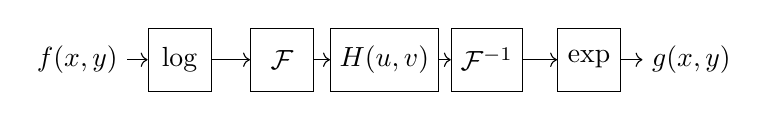
\begin{tikzpicture}[node distance=1.3cm, auto]
		% Define the style for the operation nodes
		\tikzstyle{operation}=[rectangle, draw=black, minimum size=0.8cm, text centered]

		% Define nodes
		\node (input) {$f(x,y)$};
		\node (op1) [operation, right of=input] {$\log$};
		\node (op2) [operation, right of=op1] {$\mathcal{F}$};
		\node (op3) [operation, right of=op2] {$H(u,v)$};
		\node (op4) [operation, right of=op3] {$\mathcal{F}^{-1}$};
		\node (op5) [operation, right of=op4] {$\exp$};
		\node (output) [right of=op5] {$g(x,y)$};

		% Define edges
		\draw[->] (input) -- (op1);
		\draw[->] (op1) -- (op2);
		\draw[->] (op2) -- (op3);
		\draw[->] (op3) -- (op4);
		\draw[->] (op4) -- (op5);
		\draw[->] (op5) -- (output);
	\end{tikzpicture}
	\captionof{figure}{Homomorphic filtering pipeline.}
	\label{fig:homomorphic-pipeline}
\end{figure}

Many approaches to the linear filter $H(u,v)$ exist. Voicu et al. propose to use a second order Butterworth filter \cite{voicu1997practical}, to reduce the low frequencies and enhance the high frequencies:
\begin{align}
	H(u, v) = H'(\rho) = \gamma_1  - \gamma_2 \cdot \frac{1}{1 + 2.415 \cdot \left(\frac{\rho}{\rho_c}\right)^{4}},\\
	\text{where} \qquad \rho = \sqrt{u^2 + v^2}
\end{align}
where $\gamma_H, \gamma_L, \rho_c$ are parameters that can be tuned to achieve the desired effect, and $\gamma_1 \approx \gamma_H, \gamma_2 \approx \gamma_H - \gamma_L$ \cite{voicu1997practical}. The resulting filter has the general form shown in Figure \ref{fig:homomorphic-filter}.

\begin{figure}
	\centering
	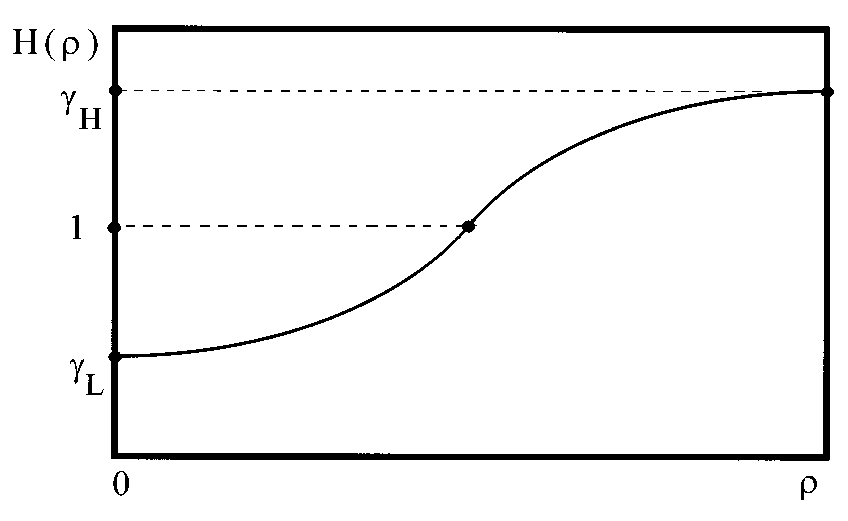
\includegraphics[width=0.45\textwidth]{images/filter.png}
	\captionof{figure}{General form of the filter used in homomorphic filtering \cite{voicu1997practical}.}
	\label{fig:homomorphic-filter}
\end{figure}

Finally, Fan et al. \cite{fan2011homomorphic} propose  to append a histogram equalization step to the homomorphic filtering pipeline, in order to improve the contrast of the image.

In order to enhance colored images using homomorphic filtering, this pipeline can be applied to a single channel, e.g. the illumination channel of HSI images, or all channels, as in RGB images. \cite{voicu1997practical,fan2011homomorphic}. An implementation of this approach is shown in Listing \ref{lst:homomorphic}.

\subsection{Evaluation of Enhancement}\label{sec:evaluation}
The quality of the enhancement can be evaluated in a few different ways. If the image was enhanced simply to improve its visual appearance, visual inspection often suffices. On the other hand, if the image was enhanced as a preprocessing step for some other computer vision task such as segmentation, the quality of the enhancement should be evaluated by measuring the performance of the computer vision task on the enhanced image. However, there are also some objective metrics that can be used to get an idea of how well an image has been enhanced:

\subsubsection{RMS Contrast}\label{sec:rms-contrast}
Contrast is a measure of the difference in brightness between the darkest and brightest parts of an image, i.e. it is a measure of how well objects are distinguishable. After enhancing an image with uneven illumination, we hope to increase the contrast in the areas of the image that originally had the same illumination. Therefore, an enhanced image might not experience a global increase in contrast, and rather some local increases. The RMS contrast is defined as the variance of the pixel intensities across the entire image \cite{dey2019uneven}:
\begin{equation}
	\text{RMS Contrast} = \frac{1}{N \cdot M} \sum_{i=1}^{N} \sum_{j=1}^{M} (I(i,j) - \bar{I})^2
\end{equation}

\subsubsection{Discrete Entropy}\label{sec:discrete-entropy}
Entropy describes the amount of information in an image, where a high entropy means that the image contains a lot of information, and a low entropy means that the image contains little information, i.e. a flat image has zero entropy. Enhancing an image with uneven illumination should increase the amount of information in the image, and therefore increase the entropy. The discrete entropy is defined as \cite{dey2019uneven,ye2007discrete}:
\begin{equation}
	\text{Discrete Entropy} = - \sum_{i} P_i \cdot \log_2(P_i)
\end{equation}
where $P_i$ is the probability that the difference between two adjacent pixels is $i$.


\section{Methodology}\label{sec:method}
In this paper we will explore the approach of stacking the three previously introduced enhancement methods into an ensemble. To do so, we utilize three separate perceptron networks, one for each color channel, in order to fuse the intermediate images produced by unsharp masking, retinex, and homomorphic filtering in pixel-wise fashion. In the following, we will describe our proposed method in detail, as well as how we trained its parameters.

\subsection{Fusion Network}\label{sec:fusion}
We investigate the stacking of unsharp masking (UM), retinex (RTX), and homomorphic filtering (HF), see Sections \ref{sec:unsharp}, \ref{sec:retinex}, and \ref{sec:homomorphic} respectively, using a simple fusion network. In particular, our pipeline undergoes the following stages: First, each of the methods will produce an intermediate enhanced image, which we will henceforth denote as $g_{UM}$, $g_{RTX}$, and $g_{HF}$. Afterwards, we will feed these images into a fusion network, to produce the final enhanced image $g_{F}$.

\begin{algorithm}
	\caption{Fusion Network}\label{alg:fusion}
	\begin{algorithmic}
	\Require $g_{UM}$, $g_{RTX}$, $g_{HF}$ in HSI color space
	\Require $w_{c} \in \mathbb{R}^3$ for $c \in \{hsi\}$
	\Ensure $N \coloneqq \text{width}(g_{UM}) = \text{width}(g_{RTX}) = \text{width}(g_{HF})$
	\Ensure $M \coloneqq \text{height}(g_{UM}) = \text{height}(g_{RTX}) = \text{height}(g_{HF})$
	\State $g_{F} \gets 0^{N \times M \times 3}$
	\For{$c \in \{hsi\}$}
		\For{$(x,y) \in \{1, \dots, N\} \times \{1, \dots, M\}$}
			\State $g_{F}(x,y,c) \gets w_{c_1} \cdot g_{UM}(x,y,c)$
			\State \qquad \qquad \qquad  $+ w_{c_2} \cdot g_{RTX}(x,y,c)$
			\State \qquad \qquad \qquad $+ w_{c_3} \cdot g_{HF}(x,y,c)$
		\EndFor
	\EndFor
	\State \Return $g_{F}$
	\end{algorithmic}
	\end{algorithm}

This fusion network consists of three separate perceptron networks, one for each of the three channels in the HSI color space. Each of these perceptrons has only three input nodes: The channel $c \in \{hsi\}$ of pixel $(x,y)$ in $g_{UM}$, $g_{RTX}$, and $g_{HF}$. The output of each perceptron is the corresponding channel of pixel $(x,y)$ in $g_{F}$. Therefore, the fusion can be described as Algorithm \ref{alg:fusion}. Here, $w_{c} \in \mathbb{R}^3$ for $c \in \{hsi\}$ are the parameters of the fusion network, which describe to what extent the intermediate images should be weighted. These parameters are learned during training, see Section \ref{sec:training}. Bias was not utilized in our experiments. The entire pipeline is also outlined in Figure \ref{fig:fusion-pipeline}.

\begin{figure}
	\centering
	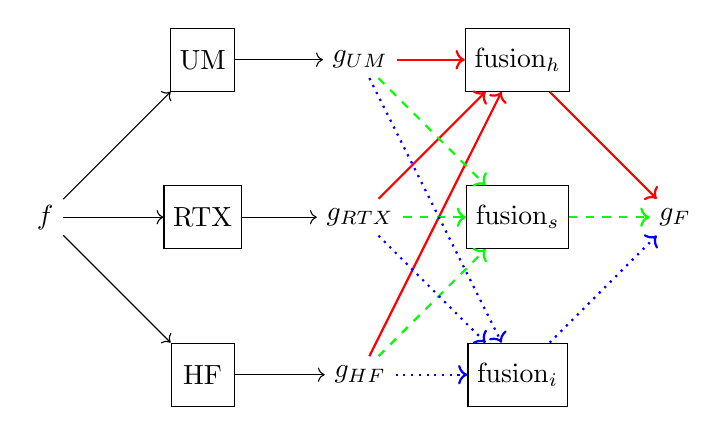
\begin{tikzpicture}[node distance=2cm, auto]
		% Define the style for the operation nodes
		\tikzstyle{operation}=[rectangle, draw=black, minimum size=0.8cm, text centered]

		% Define nodes
		\node (input) {$f$};
		\node (RTX) [operation, right of=input] {RTX};
		\node (UM) [operation, above of=RTX] {UM};
		\node (HF) [operation, below of=RTX] {HF};
		\node (g_UM) [right of=UM] {$g_{UM}$};
		\node (g_RTX) [right of=RTX] {$g_{RTX}$};
		\node (g_HF) [right of=HF] {$g_{HF}$};
		\node (H) [operation, right of=g_UM] {$\text{fusion}_h$};
		\node (S) [operation, right of=g_RTX] {$\text{fusion}_s$};
		\node (I) [operation, right of=g_HF] {$\text{fusion}_i$};
		\node (output) [right of=S] {$g_F$};

		% Define edges
		\draw[->] (input) -- (UM);
		\draw[->] (input) -- (RTX);
		\draw[->] (input) -- (HF);

		\draw[->] (UM) -- (g_UM);
		\draw[->] (RTX) -- (g_RTX);
		\draw[->] (HF) -- (g_HF);

		\draw[red,thick,arrows = {->}] (g_UM) -- (H);
		\draw[red,thick,arrows = {->}] (g_RTX) -- (H);
		\draw[red,thick,arrows = {->}] (g_HF) -- (H);
		\draw[green,thick,arrows = {->}, dashed] (g_UM) -- (S);
		\draw[green,thick,arrows = {->}, dashed] (g_RTX) -- (S);
		\draw[green,thick,arrows = {->}, dashed] (g_HF) -- (S);
		\draw[blue,thick,arrows = {->}, dotted] (g_UM) -- (I);
		\draw[blue,thick,arrows = {->}, dotted] (g_RTX) -- (I);
		\draw[blue,thick,arrows = {->}, dotted] (g_HF) -- (I);

		\draw[red,thick,arrows = {->}] (H) -- (output);
		\draw[green,thick,arrows = {->}, dashed] (S) -- (output);
		\draw[blue,thick,arrows = {->}, dotted] (I) -- (output);
	\end{tikzpicture}
	\captionof{figure}{Pipeline of the fusion network approach. Red solid arrows symbolize the fusion of the hue channel, green dashed arrows symbolize the fusion of the saturation channel, and blue dotted arrows symbolize the fusion of the intensity channel.}
	\label{fig:fusion-pipeline}
\end{figure}

\subsection{Implementation}\label{sec:implementation}
We utilized the \texttt{PyTorch}\footnote{URL: \url{https://pytorch.org/}} machine learning framework to implement the fusion network approach described in Section \ref{sec:fusion} by using three separate linear fully connected layers for each of the three color channels. A simplified implementation of the fusion network is shown in Listing \ref{lst:fusion}, while the theory and implementation of the unsharp masking, retinex, and homomorphic filtering methods is explained in Sections ref{sec:unsharp}, \ref{sec:retinex}, and \ref{sec:homomorphic} and presented in Listings \ref{lst:unsharp}, \ref{lst:retinex}, and \ref{lst:homomorphic} respectively. The full codebase of this report has been made available on GitHub\footnote{URL: \url{https://github.com/CodingTil/eiuie}}.

\begin{mdframed}[backgroundcolor=backcolour,leftmargin=0cm,hidealllines=true,innerleftmargin=0cm,innerrightmargin=0cm,innertopmargin=0cm,innerbottommargin=-0.65cm]
\lstinputlisting[language=Python, caption=Fusion Model,label=lst:fusion]{listings/fusion.py}
\end{mdframed}

\subsection{Training}\label{sec:training}
Training of the parameters $w_{c} \in \mathbb{R}^3$ for $c \in \{hsi\}$ is a crucial step for adequate enhancement. Since we are utilizing perceptron networks, we can train these parameters in a supervised learning environment. For this, we need a dataset of images with uneven illumination, as well as the corresponding ground truth images with globally even/corrected illumination. No dataset as such is known to us, and therefore we resorted to the closest alternative: the LOL-dataset consisting of image pairs taken once in low exposure (low-light), and once with normal exposure \cite{wei2018deep}.

For each image pair in the LOL-dataset, we did not only train on the low-light version as input and the normal-light image as output, but also on the normal-light image as both input and output. This way we hope that our model learns optimal parameters to not only enhance dark regions in our image with uneven illumination, but also to not over-enhance bright regions.

In total, we collected $2.4$ billion training samples (pixels). Due to memory constraints, we could only train on half of these samples. We used the Adam optimizer with a learning rate of $0.001$, and a batch size of $2^{15}$. We allowed training for $1000$ epochs, although early stopping took place shortly after epoch $100$. In total, training only took about $10$ minutes on a single NVIDIA L4 Tensor Core GPU.

\section{Results}\label{sec:results}


\section{Discussion and Conclusions}\label{sec:discussion}


%%
%% If your work has an appendix, this is the place to put it.


%%
%% The next two lines define the bibliography style to be used, and
%% the bibliography file.
\bibliographystyle{ACM-Reference-Format}
\bibliography{main}

\newpage
\appendix

\section{Listings}
\subsection{Unsharp Masking}\label{sec:unsharp-listing}
\begin{mdframed}[backgroundcolor=backcolour,leftmargin=0cm,hidealllines=true,innerleftmargin=0cm,innerrightmargin=0cm,innertopmargin=0cm,innerbottommargin=-0.65cm]
\lstinputlisting[language=Python, caption=Unsharp masking,label=lst:unsharp]{listings/unsharp_masking.py}
\end{mdframed}

\subsection{Retinex}\label{sec:retinex-listing}
\begin{mdframed}[backgroundcolor=backcolour,leftmargin=0cm,hidealllines=true,innerleftmargin=0cm,innerrightmargin=0cm,innertopmargin=0cm,innerbottommargin=-0.65cm]
\lstinputlisting[language=Python, caption=Retinex,label=lst:retinex]{listings/retinex.py}
\end{mdframed}

\subsection{Homomorphic Filtering}\label{sec:homomorphic-listing}
\begin{mdframed}[backgroundcolor=backcolour,leftmargin=0cm,hidealllines=true,innerleftmargin=0cm,innerrightmargin=0cm,innertopmargin=0cm,innerbottommargin=-0.65cm]
\lstinputlisting[language=Python, caption=Homomorphic filtering, label=lst:homomorphic]{listings/homomorphic_filtering.py}
\end{mdframed}

\end{document}
\endinput
